% Options for packages loaded elsewhere
\PassOptionsToPackage{unicode}{hyperref}
\PassOptionsToPackage{hyphens}{url}
\PassOptionsToPackage{dvipsnames,svgnames,x11names}{xcolor}
%
\documentclass[
  letterpaper,
  DIV=11,
  numbers=noendperiod]{scrartcl}

\usepackage{amsmath,amssymb}
\usepackage{lmodern}
\usepackage{iftex}
\ifPDFTeX
  \usepackage[T1]{fontenc}
  \usepackage[utf8]{inputenc}
  \usepackage{textcomp} % provide euro and other symbols
\else % if luatex or xetex
  \usepackage{unicode-math}
  \defaultfontfeatures{Scale=MatchLowercase}
  \defaultfontfeatures[\rmfamily]{Ligatures=TeX,Scale=1}
\fi
% Use upquote if available, for straight quotes in verbatim environments
\IfFileExists{upquote.sty}{\usepackage{upquote}}{}
\IfFileExists{microtype.sty}{% use microtype if available
  \usepackage[]{microtype}
  \UseMicrotypeSet[protrusion]{basicmath} % disable protrusion for tt fonts
}{}
\makeatletter
\@ifundefined{KOMAClassName}{% if non-KOMA class
  \IfFileExists{parskip.sty}{%
    \usepackage{parskip}
  }{% else
    \setlength{\parindent}{0pt}
    \setlength{\parskip}{6pt plus 2pt minus 1pt}}
}{% if KOMA class
  \KOMAoptions{parskip=half}}
\makeatother
\usepackage{xcolor}
\setlength{\emergencystretch}{3em} % prevent overfull lines
\setcounter{secnumdepth}{-\maxdimen} % remove section numbering
% Make \paragraph and \subparagraph free-standing
\ifx\paragraph\undefined\else
  \let\oldparagraph\paragraph
  \renewcommand{\paragraph}[1]{\oldparagraph{#1}\mbox{}}
\fi
\ifx\subparagraph\undefined\else
  \let\oldsubparagraph\subparagraph
  \renewcommand{\subparagraph}[1]{\oldsubparagraph{#1}\mbox{}}
\fi


\providecommand{\tightlist}{%
  \setlength{\itemsep}{0pt}\setlength{\parskip}{0pt}}\usepackage{longtable,booktabs,array}
\usepackage{calc} % for calculating minipage widths
% Correct order of tables after \paragraph or \subparagraph
\usepackage{etoolbox}
\makeatletter
\patchcmd\longtable{\par}{\if@noskipsec\mbox{}\fi\par}{}{}
\makeatother
% Allow footnotes in longtable head/foot
\IfFileExists{footnotehyper.sty}{\usepackage{footnotehyper}}{\usepackage{footnote}}
\makesavenoteenv{longtable}
\usepackage{graphicx}
\makeatletter
\def\maxwidth{\ifdim\Gin@nat@width>\linewidth\linewidth\else\Gin@nat@width\fi}
\def\maxheight{\ifdim\Gin@nat@height>\textheight\textheight\else\Gin@nat@height\fi}
\makeatother
% Scale images if necessary, so that they will not overflow the page
% margins by default, and it is still possible to overwrite the defaults
% using explicit options in \includegraphics[width, height, ...]{}
\setkeys{Gin}{width=\maxwidth,height=\maxheight,keepaspectratio}
% Set default figure placement to htbp
\makeatletter
\def\fps@figure{htbp}
\makeatother

\KOMAoption{captions}{tableheading}
\makeatletter
\makeatother
\makeatletter
\makeatother
\makeatletter
\@ifpackageloaded{caption}{}{\usepackage{caption}}
\AtBeginDocument{%
\ifdefined\contentsname
  \renewcommand*\contentsname{Table of contents}
\else
  \newcommand\contentsname{Table of contents}
\fi
\ifdefined\listfigurename
  \renewcommand*\listfigurename{List of Figures}
\else
  \newcommand\listfigurename{List of Figures}
\fi
\ifdefined\listtablename
  \renewcommand*\listtablename{List of Tables}
\else
  \newcommand\listtablename{List of Tables}
\fi
\ifdefined\figurename
  \renewcommand*\figurename{Figure}
\else
  \newcommand\figurename{Figure}
\fi
\ifdefined\tablename
  \renewcommand*\tablename{Table}
\else
  \newcommand\tablename{Table}
\fi
}
\@ifpackageloaded{float}{}{\usepackage{float}}
\floatstyle{ruled}
\@ifundefined{c@chapter}{\newfloat{codelisting}{h}{lop}}{\newfloat{codelisting}{h}{lop}[chapter]}
\floatname{codelisting}{Listing}
\newcommand*\listoflistings{\listof{codelisting}{List of Listings}}
\makeatother
\makeatletter
\@ifpackageloaded{caption}{}{\usepackage{caption}}
\@ifpackageloaded{subcaption}{}{\usepackage{subcaption}}
\makeatother
\makeatletter
\@ifpackageloaded{tcolorbox}{}{\usepackage[many]{tcolorbox}}
\makeatother
\makeatletter
\@ifundefined{shadecolor}{\definecolor{shadecolor}{rgb}{.97, .97, .97}}
\makeatother
\makeatletter
\makeatother
\ifLuaTeX
  \usepackage{selnolig}  % disable illegal ligatures
\fi
\IfFileExists{bookmark.sty}{\usepackage{bookmark}}{\usepackage{hyperref}}
\IfFileExists{xurl.sty}{\usepackage{xurl}}{} % add URL line breaks if available
\urlstyle{same} % disable monospaced font for URLs
\hypersetup{
  pdftitle={Data Management \& Programming Project},
  pdfauthor={Adrien BOUISSON \& Ghina MEZHER},
  colorlinks=true,
  linkcolor={blue},
  filecolor={Maroon},
  citecolor={Blue},
  urlcolor={Blue},
  pdfcreator={LaTeX via pandoc}}

\title{Data Management \& Programming Project}
\author{Adrien BOUISSON \& Ghina MEZHER}
\date{}

\begin{document}
\maketitle
\ifdefined\Shaded\renewenvironment{Shaded}{\begin{tcolorbox}[sharp corners, borderline west={3pt}{0pt}{shadecolor}, frame hidden, enhanced, breakable, interior hidden, boxrule=0pt]}{\end{tcolorbox}}\fi

\hypertarget{our-research-question}{%
\section{Our research question}\label{our-research-question}}

\hypertarget{i.-the-importance-and-history-of-research-in-education}{%
\subsection{I. The importance and history of research in
education}\label{i.-the-importance-and-history-of-research-in-education}}

It is undeniable education profoundly shapes societal progress. From
allowing humans to make world changing discoveries to multiplying the
efficiency and use of physical capital; education lets each individual
make use of their production power. Education is also considered a
fundamental right, as it is stipulated in the universal declaration of
Human Rights 1948, and a key element of development as seen in the 2000
MDGs (MDG n°2) and the 2015 SDGs (SDG n°4).

Today, economic research in education is considered a greatly developed
field, highlighting the importance of public spending in education and
the necessity for targeted funding and strategic policies. We owe the
establishment of the field to the theory of human capital by Schultz,
Becker and Mincer established in the 50's . What started as a simple
causality relationship between additional years of education and wage
differences was frivolously applied to empirical studies, and
econometric models. This allowed researchers to understand countries'
particular attributes and situations but also if lack of education
should be considered a demand or a supply problem.

Investing in human capital, here in its educational form, is considered
fundamental to the reduction of inequalities. Take for example woman's
fertility. Research has found that, in developing countries, one
additional year of schooling reduces woman's fertility rate by 10\%,
enabling a much needed demographic transition. This causality
relationship can be explained by the increase of revenue on the labor
market through additional years of schooling, allowing women to take on
better jobs and increasing the opportunity cost of having a child.

\hypertarget{ii.-the-link-between-education-and-unemployment}{%
\subsection{II. The link between education and
unemployment}\label{ii.-the-link-between-education-and-unemployment}}

The polarization of the labor market has become a clear and urgent
issue. The dreaded phenomenon represents, for the middle class, the end
of social mobility. Polarization of the labor market defines the
historical decline of the rate of jobs that lie in the middle of the
distribution of qualification (France Stratégie 2020). The prosperity of
machinery and innovation has led to the decrease of basic qualification
demanding jobs in favor of highly qualified jobs or low qualified jobs.
This phenomenon has revealed itself particularly challenging for
under-qualified youth, whose unemployment rate has increased in the past
few years.

In order to form the subject of our study we begun with the same idea as
the theory of capital : how can altering the offer of education impacts
individuals' status on the labor market.

However, in a will to understand the role the government must play when
it comes to the offer in education we may ask ourselves : Should
government leaders expect their educational spending to impact the
unemployment rate ?

A higher unemployment rate could also prompt governments to allocate
more funds to education as a way to respond to the need for training to
boost employability, we therefore see a potential double causality
between educational spending and unemployment. The potential reciprocal
influence between educational investments and workforce participation
unveils a complex interplay, emphasizing the need for nuanced analysis
to comprehend the multifaceted impact of education on labor markets.

Ultimately, this exploration aims to inform policy decisions, offering
insights into the interwoven pathways that shape both educational
outcomes and employment prospects, fostering more holistic approaches
towards societal development.

All these elements lead us to ask the following question: How can public
spending on education help reduce youth unemployment in the world?

To answer our question, we will first look at the general trends in
public spending and youth unemployment since 1970. We will then show
that education spending is essential to reducing youth unemployment.
Finally, we'll see that this is not enough, and that the reduction in
the unemployment rate is made possible by other factors such as the
country's development, rigidity on the labor market, etc.

\hypertarget{data-set-description}{%
\section{Data set description}\label{data-set-description}}

Our topic of study in this project tackles the impact of education
spending on the youth unemployment rate. For that, we have decided to
take our databases from sites such as the World Bank and the
International Labor Organization (ILO), as these are major global
institutions known primarily for their availability and accessibility.
For example, World Bank compiles and makes available a wide range of
data on global economic development such as expenditures in school per
country.

Thanks to the richness of information in our panel ILO data base and
panel World Bank database we will be able to study the impact of public
educational spending on the educational aspect of human capital. With
the detailed information from various countries and on a big date range,
we are able to study the impact on a micro and macro level. The micro
impact can be observed by studying each country on its own and observing
the variations throughout the years. This also makes comparing countries
possible; we could therefore observe the impact on developing countries
and developed countries. We can also compare the effects of education
spending on the youth unemployment rate within countries, i.e.~between
men and women, and between countries, i.e.~the macroeconomic impact of
education spending.

We would like to highlight the real and empirical impact of the
augmentation of educational spending on level of education thanks to the
``classif2'' variable now called ``Education''. Through this potential
correlation and causality we could understand the impact of a budgetary
politic in education on unemployment. The underlying assumption is that
a positive correlation between increased educational spending and higher
education levels could translate into a subsequent decline in
unemployment figures over the ensuing years. Therefore the project
endeavors to decipher how these factors (public spending and education
levels) interplay in the context of unemployment rates.

Our databases are dense, which requires delimiting our subject such as
the period on which we are going to be studying or the variables that we
consider to be most relevant.

\hypertarget{description-of-the-world-bank-database}{%
\subsection{Description of the World bank
database}\label{description-of-the-world-bank-database}}

First, many of the databases provided by the World Bank include time
series data, allowing to analyze trends and changes over time. It could
be essential for understanding the dynamics of variables. Then, the
World Bank is known for maintaining high standards in databases. There
is data reliability, World Bank data is generally subject to rigorous
standards and quality controls. As part of our project, the database
from the World Bank allows us to make international comparisons by
collecting data from many countries, such as school expenditure for
example.

Finally, by analyzing World Bank data on school expenditures, we can
merge this database with the youth unemployment rate to study the
correlation (or causality) of education spending on the unemployment
rate.

It means that we could observe that the higher education spending led to
a lower youth unemployment rate, or that the high youth unemployment
rate can be explained by lower spending on education.

\hypertarget{table-1.-description-of-our-wb-database}{%
\subsubsection{Table 1. Description of our WB
database}\label{table-1.-description-of-our-wb-database}}

\begin{longtable}[]{@{}
  >{\raggedright\arraybackslash}p{(\columnwidth - 10\tabcolsep) * \real{0.1579}}
  >{\raggedright\arraybackslash}p{(\columnwidth - 10\tabcolsep) * \real{0.0902}}
  >{\raggedleft\arraybackslash}p{(\columnwidth - 10\tabcolsep) * \real{0.1880}}
  >{\raggedright\arraybackslash}p{(\columnwidth - 10\tabcolsep) * \real{0.4060}}
  >{\raggedright\arraybackslash}p{(\columnwidth - 10\tabcolsep) * \real{0.0827}}
  >{\raggedright\arraybackslash}p{(\columnwidth - 10\tabcolsep) * \real{0.0752}}@{}}
\toprule()
\begin{minipage}[b]{\linewidth}\raggedright
Origin
\end{minipage} & \begin{minipage}[b]{\linewidth}\raggedright
Last update
\end{minipage} & \begin{minipage}[b]{\linewidth}\raggedleft
Nb of countries observed
\end{minipage} & \begin{minipage}[b]{\linewidth}\raggedright
Indicator
\end{minipage} & \begin{minipage}[b]{\linewidth}\raggedright
First date
\end{minipage} & \begin{minipage}[b]{\linewidth}\raggedright
Last date
\end{minipage} \\
\midrule()
\endhead
Table 1 : World bank & 2023-10-26 & 266 & Government expenditure on
education, total (\% of GDP) & 1960 & 2022 \\
\bottomrule()
\end{longtable}

\hypertarget{variable-description}{%
\paragraph{Variable description}\label{variable-description}}

\begin{itemize}
\item
  ``Country Name''/``Country Code'': String value giving us an indicator
  for each country to classify values
\item
  ``Indicator Name''/``Indicator code'': String value giving us the
  indicator studied wich is the government expenditure on education as
  \% of GDP
\item
  ``Date'': each column referring to a date for the \% of GDP for
  government education spending going from 1960 to 2022
\end{itemize}

\hypertarget{description-of-the-international-labor-organisation-database}{%
\subsection{Description of the International Labor Organisation
database}\label{description-of-the-international-labor-organisation-database}}

Then, the International Labor Organization (ILO) provides a wealth of
data related to labor and employment. The ILO sets international
standards for labor and labor statistics. These standards guarantee a
consistent methodology for the collection and presentation of data on
the labor market, including the unemployment rate.This site therefore
corresponds perfectly to our project.

ILO data offers comprehensive insights into the global labor marker,
especially unemployment in the world, and youth unemployment (15-29
years old). Like the World Bank, the ILO collects and compiles data on
youth unemployment from a wide range of countries, allowing for
international comparisons which is perfect for our project. Both sites
making international comparisons, it allows for an interesting world
level analysis of our subject of study.

\hypertarget{table-2.-description-of-our-ilo-database}{%
\subsubsection{Table 2. Description of our ILO
database}\label{table-2.-description-of-our-ilo-database}}

\begin{longtable}[]{@{}
  >{\raggedright\arraybackslash}p{(\columnwidth - 14\tabcolsep) * \real{0.1321}}
  >{\raggedleft\arraybackslash}p{(\columnwidth - 14\tabcolsep) * \real{0.1509}}
  >{\raggedleft\arraybackslash}p{(\columnwidth - 14\tabcolsep) * \real{0.1509}}
  >{\raggedleft\arraybackslash}p{(\columnwidth - 14\tabcolsep) * \real{0.1038}}
  >{\raggedleft\arraybackslash}p{(\columnwidth - 14\tabcolsep) * \real{0.1132}}
  >{\raggedleft\arraybackslash}p{(\columnwidth - 14\tabcolsep) * \real{0.1509}}
  >{\raggedleft\arraybackslash}p{(\columnwidth - 14\tabcolsep) * \real{0.1038}}
  >{\raggedleft\arraybackslash}p{(\columnwidth - 14\tabcolsep) * \real{0.0943}}@{}}
\toprule()
\begin{minipage}[b]{\linewidth}\raggedright
Origin
\end{minipage} & \begin{minipage}[b]{\linewidth}\raggedleft
Nb of variables
\end{minipage} & \begin{minipage}[b]{\linewidth}\raggedleft
Nb of countries
\end{minipage} & \begin{minipage}[b]{\linewidth}\raggedleft
Sex groups
\end{minipage} & \begin{minipage}[b]{\linewidth}\raggedleft
Age groups
\end{minipage} & \begin{minipage}[b]{\linewidth}\raggedleft
Number of dates
\end{minipage} & \begin{minipage}[b]{\linewidth}\raggedleft
First date
\end{minipage} & \begin{minipage}[b]{\linewidth}\raggedleft
Last date
\end{minipage} \\
\midrule()
\endhead
Table 2 : ILO & 12 & 167 & 4 & 4 & 37 & 1987 & 2023 \\
\bottomrule()
\end{longtable}

\hypertarget{main-variables-description}{%
\subsubsection{Main variables
description}\label{main-variables-description}}

``Ref area'': String value giving us each country's code, for example
``AFG'' for Afghanistan. It can refer to countries, geographic regions,
groups of countries (by income level or others) or the world

``sex'': string value giving us the sex, three categories: total, male,
female \& other. The breakdown by sex and the items of this breakdown.

``classif1'': string value giving us the youth range, three categories:
15-19, 20-24, 25-29, 15-29, for example ``AGE\_YTHBANDS\_Y15-29'',``Age
(Tranches des jeunes): 15-29''

``classif2'': string value giving us the level of education of observed
category, 6 categories are mentioned: Total (values for all categories),
Less than basic, basic, intermediate, advanced and level not stated

``time'': string value giving us the date of the observation

``obs\_value'': observed value according to each category

\hypertarget{table-3.-a-summary-of-our-merged-and-cleaned-database}{%
\subsubsection{Table 3. A summary of our merged and cleaned
database}\label{table-3.-a-summary-of-our-merged-and-cleaned-database}}

We've merged our 2 databases in order to match them by country (variable
``Country'') and date (variable ``time'').

\begin{longtable}[]{@{}
  >{\raggedright\arraybackslash}p{(\columnwidth - 10\tabcolsep) * \real{0.5132}}
  >{\raggedleft\arraybackslash}p{(\columnwidth - 10\tabcolsep) * \real{0.1250}}
  >{\raggedleft\arraybackslash}p{(\columnwidth - 10\tabcolsep) * \real{0.1053}}
  >{\raggedleft\arraybackslash}p{(\columnwidth - 10\tabcolsep) * \real{0.1053}}
  >{\raggedleft\arraybackslash}p{(\columnwidth - 10\tabcolsep) * \real{0.0724}}
  >{\raggedright\arraybackslash}p{(\columnwidth - 10\tabcolsep) * \real{0.0789}}@{}}
\toprule()
\begin{minipage}[b]{\linewidth}\raggedright
Title
\end{minipage} & \begin{minipage}[b]{\linewidth}\raggedleft
Nb of observations
\end{minipage} & \begin{minipage}[b]{\linewidth}\raggedleft
Nb of variables
\end{minipage} & \begin{minipage}[b]{\linewidth}\raggedleft
Nb of countries
\end{minipage} & \begin{minipage}[b]{\linewidth}\raggedleft
Age groups
\end{minipage} & \begin{minipage}[b]{\linewidth}\raggedright
Time frame
\end{minipage} \\
\midrule()
\endhead
Table 3 : Education spending and youth unemployment rate by country over
time & 108988 & 7 & 162 & 4 & 1987 - 2022 \\
\bottomrule()
\end{longtable}

\hypertarget{data-analysis}{%
\section{Data Analysis}\label{data-analysis}}

\hypertarget{i.-public-spending-and-youth-unemployment-in-the-world}{%
\subsection{I. Public spending and youth unemployment in the
world}\label{i.-public-spending-and-youth-unemployment-in-the-world}}

\hypertarget{public-spending-on-education-since-2014-in-the-world}{%
\subsubsection{1) Public spending on education since 2014 in the
world}\label{public-spending-on-education-since-2014-in-the-world}}

To begin our analysis, we'll be looking at how public spending on
education has evolved around the world. This will enable us to look at
general trends, and to see which countries have the highest and lowest
educational expenditure.

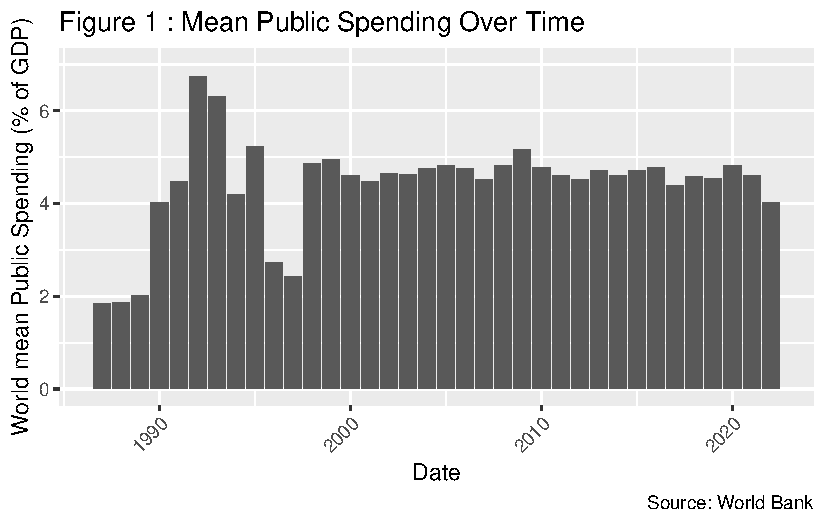
\includegraphics{Projet-BM_files/figure-pdf/unnamed-chunk-9-1.pdf}

Therefore we can see public spending varies through time with a
particular low in 1996 and 1997. Over the past few years, the average
public spending on education has hovered around 4.8\% of GDP with a
decline starting 2021; we might imagine a reorientation of public
spending to other sectors like health, security and energy following the
pandemic and the war in Ukraine. It is therefore interesting to conduct
a more in depth examination of public expenditure trends since 2014, in
order to define which countries contribute to elevating this average and
those that contribute to lowering it.

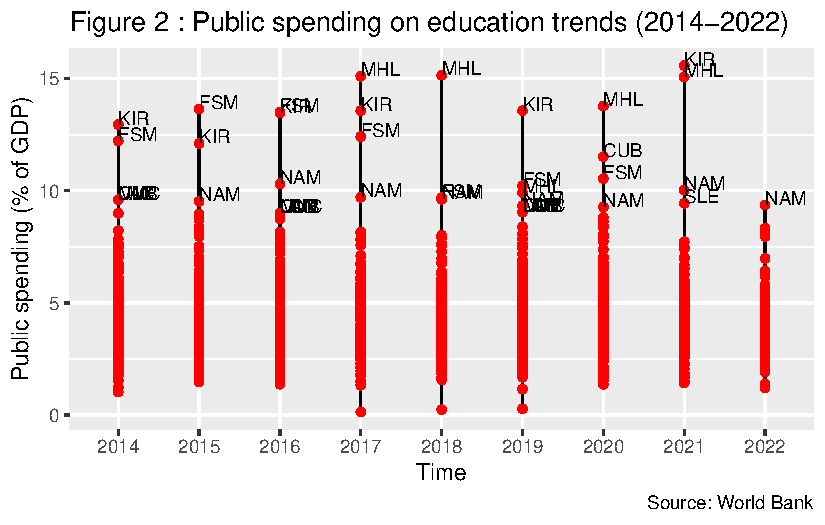
\includegraphics{Projet-BM_files/figure-pdf/unnamed-chunk-10-1.pdf}

Thanks to this graph, we have the evolution of public spending on
education over the period 2014-2022. The dots represent the countries,
we can therefore see that the average public expenditure in 2021 is
elevated by Kiribati and the Marshall Islands' public spending on
education. These two countries have also relatively high education
spending in the 2014-2022 time span, also adding to that list Namibia
and the Federated States of Micronesia. Therefore examining the
influence of public spending on the youth unemployment rate in countries
situated in Africa (for the case of Namibia) would be a compelling study
taking into account that the MDGs and SDGs on education focused on
development projects in the region.

\hypertarget{a-the-largest-share-of-gdp-for-public-spending-in-education}{%
\subsubsection{a) The largest share of GDP for public spending in
education}\label{a-the-largest-share-of-gdp-for-public-spending-in-education}}

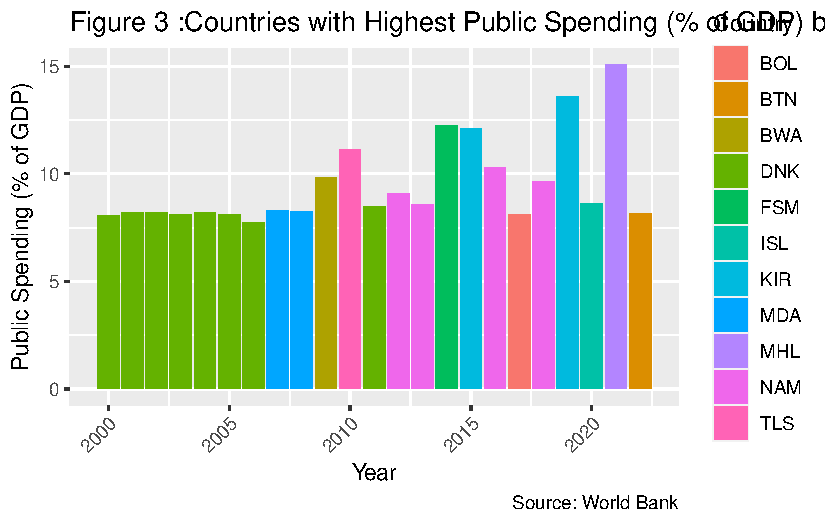
\includegraphics{Projet-BM_files/figure-pdf/unnamed-chunk-11-1.pdf}

Countries that devote a large share of their GDP to education spending
are : Samoa américaines (ASM), Cuba (CUB), Micronésie, Etats fédérés
(FSM), Kiribati (KIR), Lesotho (LS0), Marshall's Islands (MHL), Namibie
(NAM).

\hypertarget{b-the-smallest-share-of-gdp-for-public-spending}{%
\subsubsection{b) The smallest share of GDP for public
spending}\label{b-the-smallest-share-of-gdp-for-public-spending}}

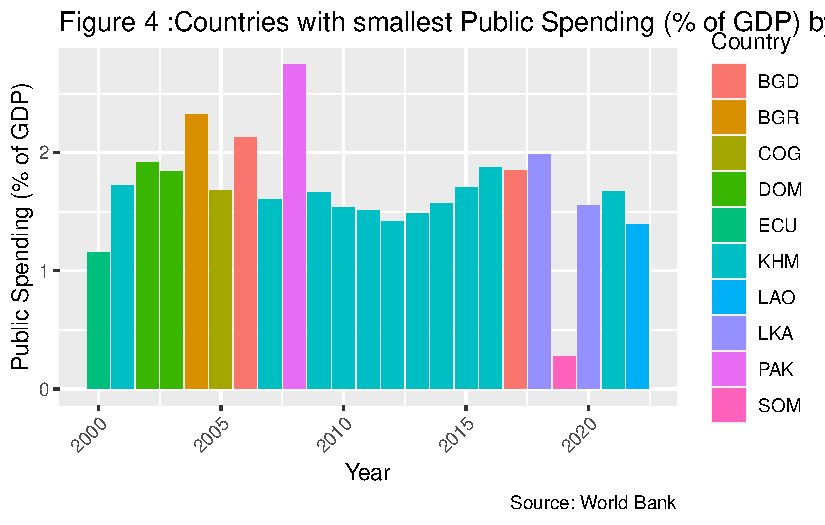
\includegraphics{Projet-BM_files/figure-pdf/unnamed-chunk-12-1.pdf}

Countries that devote a large share of their GDP to education spending
are : Africa Eastern and Southern (AFE), Central African Republic (CAF),
Zambia (ZMB), South Sudan (SSD), Sudan (SDN), Gambia (GMB), etc.. The
majority of countries that spend the least on education are in Africa,
this only highlights the need to understand the efficiency of public
expenditure in the region in order to orientate public policy and
spending towards the education field.

\hypertarget{youth-unemployment-in-the-world}{%
\subsubsection{2) Youth unemployment in the
world}\label{youth-unemployment-in-the-world}}

In this section, we'll take a look at the evolution of the global youth
unemployment rate over the period 2014-2022. Taking the same period as
public spending will allow us to account for a potential correlation (or
even causality) between public spending and the unemployment rate in a
second part. Here, we analyze only the major trends to begin our study.

Unemployment refers to the deprivation of a job. An unemployed person is
not deprived of work, but of employment. For the person who holds it,
employment is a source of income through participation in the economic
distribution of the wealth produced.

According to ILO, an unemployed person is a person aged 15 or over who
simultaneously meets three conditions: being unemployed during a given
week; being available to take up a job within two weeks; having actively
looked for a job in the last four weeks or having found one starting in
less than three months.

In the wake of worsening youth unemployment in Europe, a debate has
recently emerged about the instrument used at the ILO: should rates or
ratios be used to express youth unemployment?

The difference lies in the denominator: only the young workforce - those
working or looking for work - is taken into account in the case of the
rate, as opposed to the entire 15-24 age group - including full-time
students - in the case of the ratio.

So, if we look at 200 young people, 100 of whom are students and 50
employed, the unemployment rate is 50 percent, while the ratio is 25
percent.

Applying a ratio can be useful for comparing levels of youth
unemployment between countries, because there are significant
differences in the way countries count youth participation in the
workforce. In the case of ILO database we have a unemployment rate which
enables us to compare countries in our database.

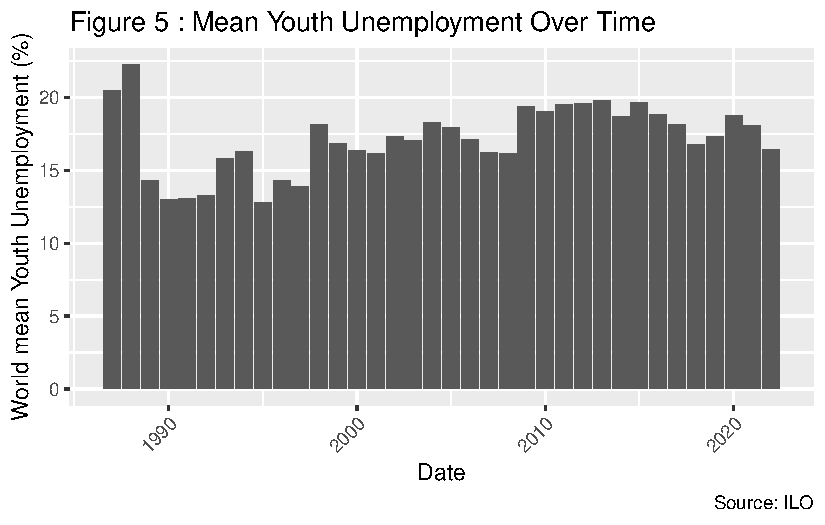
\includegraphics{Projet-BM_files/figure-pdf/unnamed-chunk-13-1.pdf}

We can see that the global youth unemployment rate has been rising for
several decades with a decrease since 2020, focusing on that time frame
allows us to understand if this decrease is led by an increase in public
spending in education.

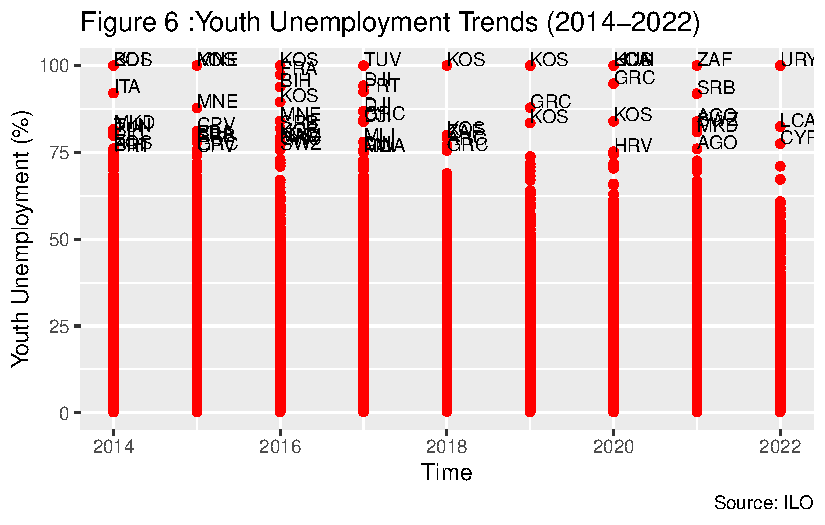
\includegraphics{Projet-BM_files/figure-pdf/unnamed-chunk-14-1.pdf}

Through this graph we can see countries with highest youth unemployment
rate at the top of the line. They are Kosovo, South Africa,
Uruguay,Tuvalu and Greece. They do not appear as countries who spend the
lowest \% of GDP on education, it is therefore interesting to conduct a
study on African countries in order to understand the potential
causality or non-causality between public expenditure and youth
unemployment.

\hypertarget{a-the-highest-youth-unemployment-rate---15-19-20-24-years-old}{%
\subsubsection{a) The highest youth unemployment rate - 15-19 \& 20-24
years
old}\label{a-the-highest-youth-unemployment-rate---15-19-20-24-years-old}}

Having seen which countries devote the most or least of their GDP to
education spending, we're now going to look at which countries have the
highest and lowest unemployment rates among young people, in this case
15-24 year-old.

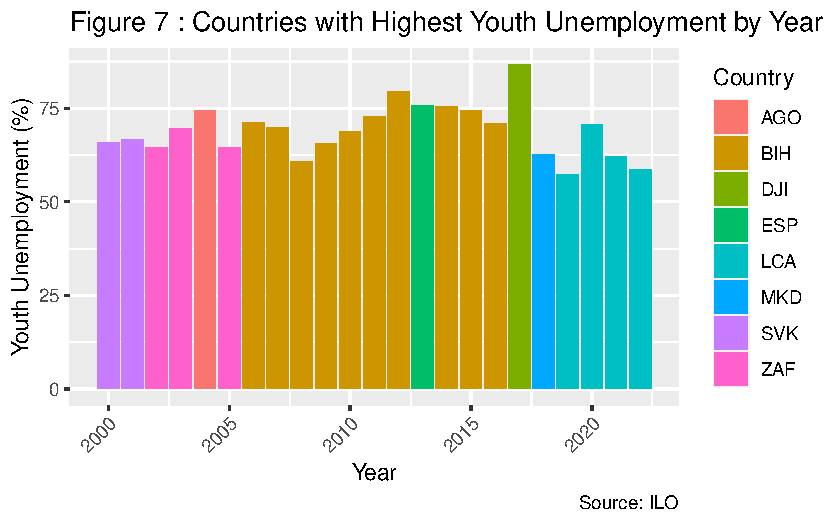
\includegraphics{Projet-BM_files/figure-pdf/unnamed-chunk-15-1.pdf}

Countries with the highest youth unemployment rates are : Angola (AGO),
Bosnia and Herzegovina (BIH), Djibouti (DJI), Spain (ESP), Saint Lucia
(LCA), North Macedonia (MKD), South Africa (ZAF).

\hypertarget{b-the-lowest-youth-unemployment-rate---15-19-20-24-years-old}{%
\subsubsection{b) The lowest youth unemployment rate - 15-19 \& 20-24
years
old}\label{b-the-lowest-youth-unemployment-rate---15-19-20-24-years-old}}

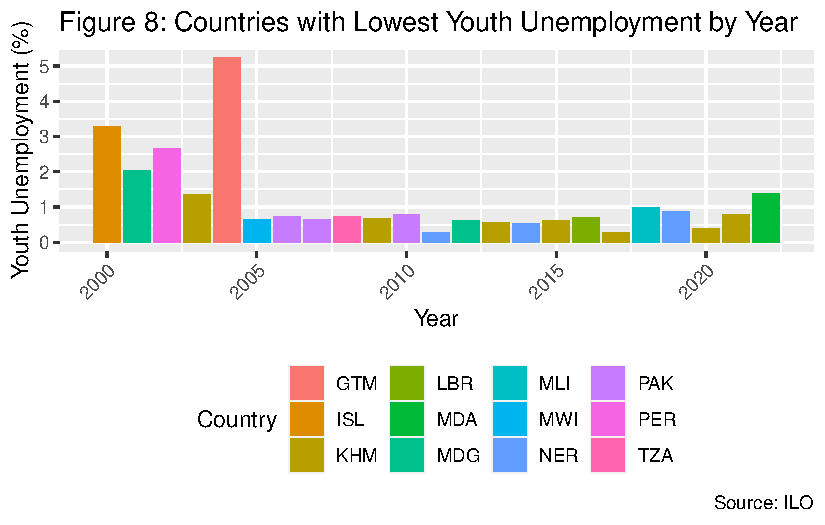
\includegraphics{Projet-BM_files/figure-pdf/unnamed-chunk-16-1.pdf}

Countries with the lowest youth unemployment rates are : Switzerland
(CHE), Guatemala (GTM), Cambodia (KHM), Liberia (LBR), Moldova (MDA),
Madagascar (MDG), Mali (MLI), Malawi (MWI), Niger (NER), Pakistan (PAK),
Peru (PER), Rwanda (RWA).

We can see from this graph that the place where youth unemployment is
highest is predominantly in Africa. Public spending can therefore have
an impact on the youth unemployment rate. But we can also see that some
African countries have the lowest unemployment rates, so education
spending isn't the only explanatory variable.

\hypertarget{general-observation-of-public-spending-in-education-and-youth-unemployment}{%
\subsubsection{3) General observation of public spending in education
and youth
unemployment}\label{general-observation-of-public-spending-in-education-and-youth-unemployment}}

In order to have a more in depth analysis of general trends and
understand the different impact of public expenditure on sexes, age
groups and level of education we must select one year to study out of
our panel data. The code becomes quite simple to alter in order to study
another date by replacing the year 2021 that we have chosen with
whichever year is of interest to the researcher.

We have chosen the year 2021 as it is the year where public expenditure
and youth unemployment started to recede. As we have only observed world
averages it would be interesting to have a more in depth look at some
countries to better understand these trends and how they apply to
different categories and regions. Add onto that the high public spending
of some countries that year, we will be able to observe their impact on
youth unemployment according to sex and level of education.

\hypertarget{a-general-observations}{%
\paragraph{a) General observations}\label{a-general-observations}}

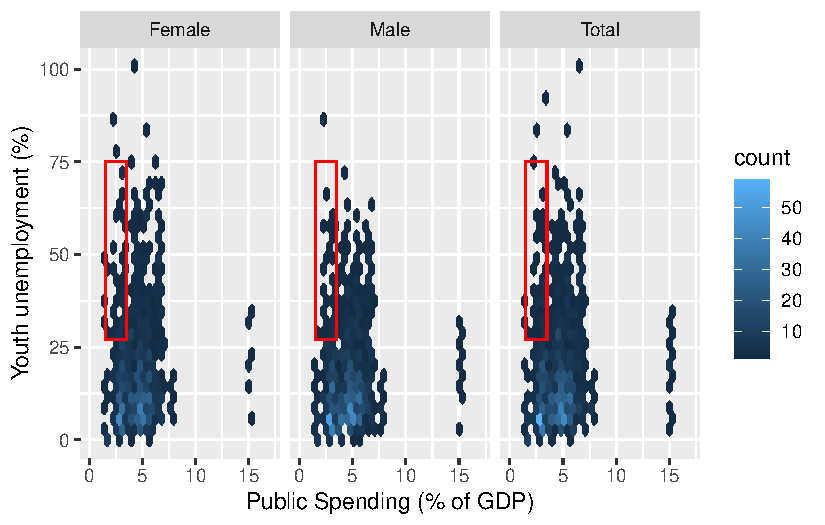
\includegraphics{Projet-BM_files/figure-pdf/unnamed-chunk-17-1.pdf}

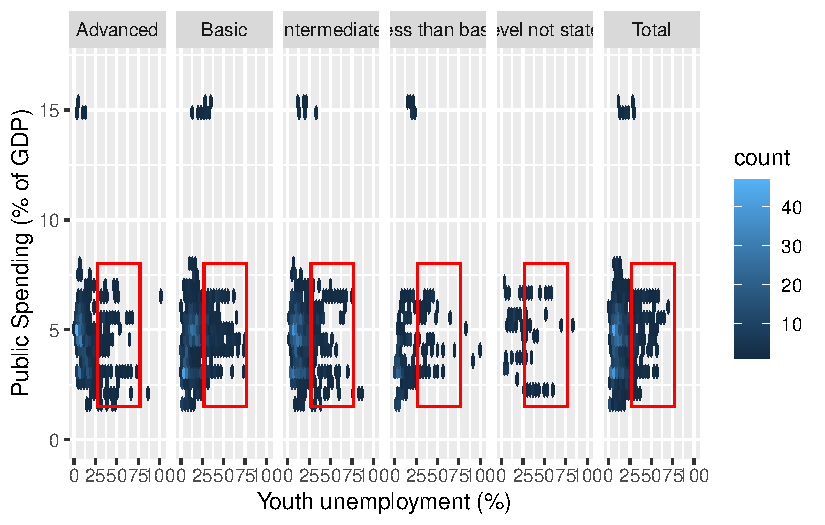
\includegraphics{Projet-BM_files/figure-pdf/unnamed-chunk-17-2.pdf}

We can therefore see a small disparity in the distribution of points
between the subplots of each of these two graphs. When it comes to the
genders, women tend to have a higher youth unemployment rate than men
for the same public spending in \% of GDP. When it comes to level of
education, for the same amount of public spending in education, the
youth unemployment rate tends to be higher for a level of education
stated as ``Basic'' than ``Advanced''. More education seems to be a good
way to reduce unemployment. Public spending can therefore be a useful
tool to push students to achieve an advanced level of education,
reducing the unemployment rate the year they enter the labor market.

Take for example countries with high public spending. They tend to have
an overall lower youth unemployment rate (especially for an advanced
level of education) might it be for the different sexes or level of
education. The disparity in youth unemployment between men and women and
different levels of education is less prominent for countries with
higher public spending.

The graphs remain quite hard to read as each point represents one
country for one age range, it is therefore interesting to take on the
analysis of certain representative countries for each of our later
sections to better see how public spending in education impacts men and
women differently.

\hypertarget{b-impact-of-public-spending-on-education-level}{%
\paragraph{b) impact of public spending on education
level}\label{b-impact-of-public-spending-on-education-level}}

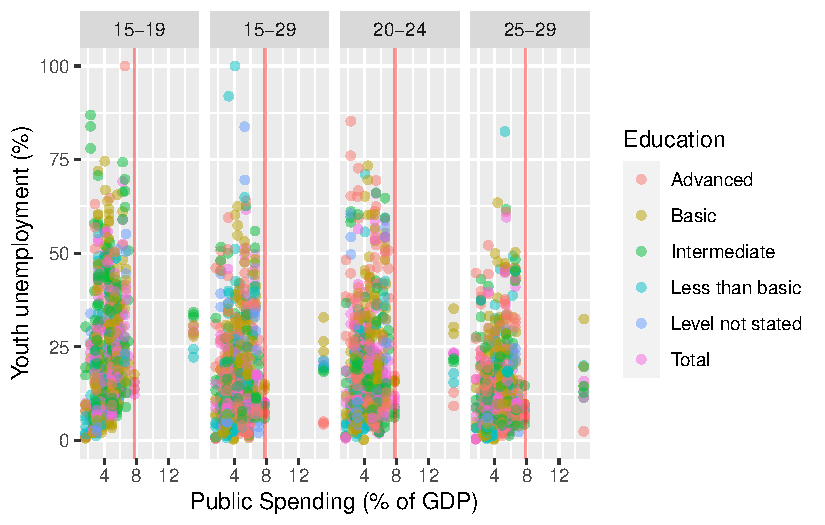
\includegraphics{Projet-BM_files/figure-pdf/unnamed-chunk-18-1.pdf}

This general observation allows us to take into account the impact of
public spending on education by Age groups and by level of education,
for the year 2021.

Generally, a higher public spending rate allows for lower youth
unemployment on all age ranges. For a relatively high public spending
(around 7\%) we can see an ``Advanced'' red dot with a 100\% youth
unemployment rate. This could be due to the use of the ratio of youth
unemployment counting students as unemployed. For this specific case,
the 100\% unemployment ratio might be led by a large part of 15-19 years
pursuing higher education thanks to good public expenditure.

In order to read this graph we could take a look at a specific value of
Public Spending, for example 7.8\% of GDP. This is considered a high
public spending in education. We can therefore see which levels of
education are benefiting from this public expenditure. We can see that
for such a public spending and for the different age ranges, advanced
level of education tends to have a lower youth unemployment rate.

Public spending therefore impacts individuals differently and according
to their level of education. An individual that has an intermediate
level at 15-19 and gets on the labor market will not benefit from the
public expenditure. This is why for countries with higher public
spending we can see the points tend to stay lower as public expenditure
promotes and helps individuals stay in the school system.

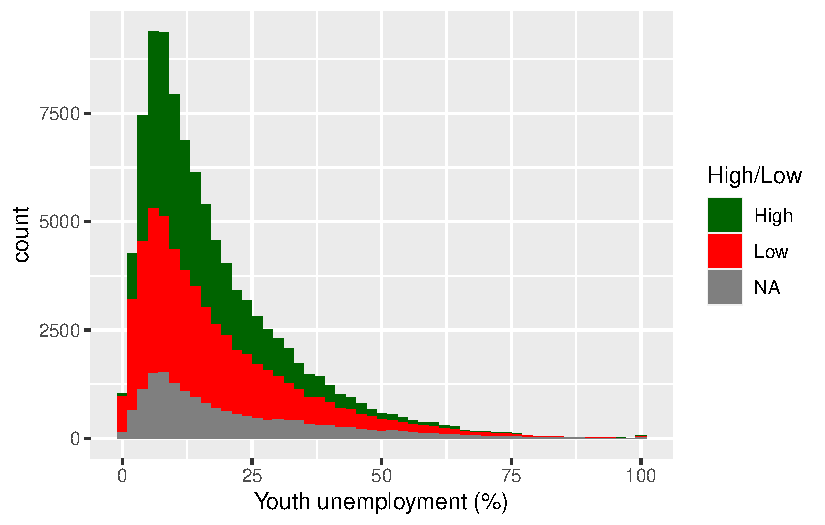
\includegraphics{Projet-BM_files/figure-pdf/unnamed-chunk-19-1.pdf}

Here we divided our observations into 2 sections thanks to the creation
of a High/Low dummy variable. Countries with ``High'' public spending in
education have a \% of GDP dedicated to education superior to the mean
of our database. Here we can see that as youth unemployment rises, the
count of countries with a high public spending decreases becoming
smaller than the red bars that represent ``Low'' spending in education.

\hypertarget{ii.-public-spending-and-youth-unemployment-in-developed-countries}{%
\subsection{II. Public spending and youth unemployment in developed
countries}\label{ii.-public-spending-and-youth-unemployment-in-developed-countries}}

Counter-intuitively, developed countries do not allocate the highest \%
of GDP to public spending on education.

We'll be looking at public spending trends in developed countries such
as the United States, France, Germany, Japan, Canada, the United
Kingdom, Russia and Italy.

\hypertarget{public-spending-in-education-in-developed-countries-g8-countries}{%
\subsubsection{1) PUblic spending in education in developed countries:
G8
countries}\label{public-spending-in-education-in-developed-countries-g8-countries}}

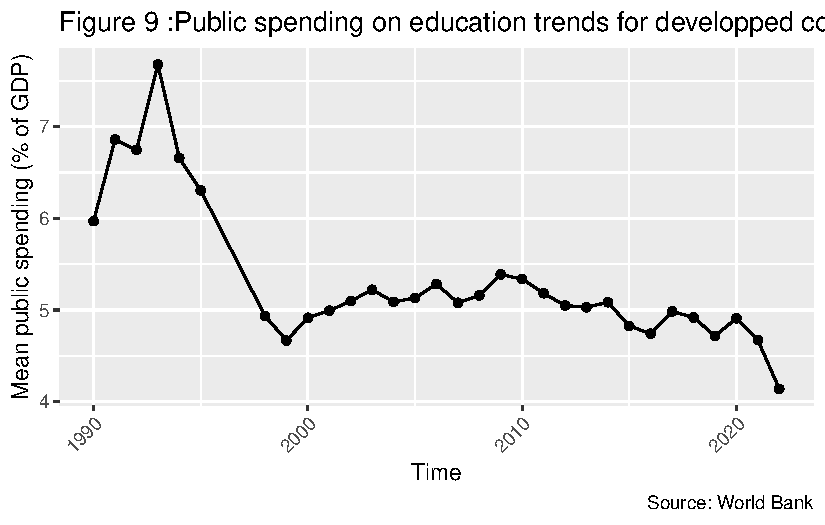
\includegraphics{Projet-BM_files/figure-pdf/unnamed-chunk-20-1.pdf}

Since the 1970s, there has been a general decline trend in education
spending in the G8 countries. This decline can be explained by the aging
of the population, leading to a reallocation of public spending to
health. Another factor may be government priorities. The sudden increase
in 1993 can be explained by the fall of the Berlin Wall and the end of
the Cold War, which reduced trade between countries and hence GDP. As
education spending remained unchanged, its share of GDP increased. In
2020, the decline in the share of education spending fell sharply as a
result of the health crisis, which reduced both GDP and education
spending.

Moreover, this graph plots the average for G8 countries without taking
into account the disparities between them, as we shall see in the
following graph.

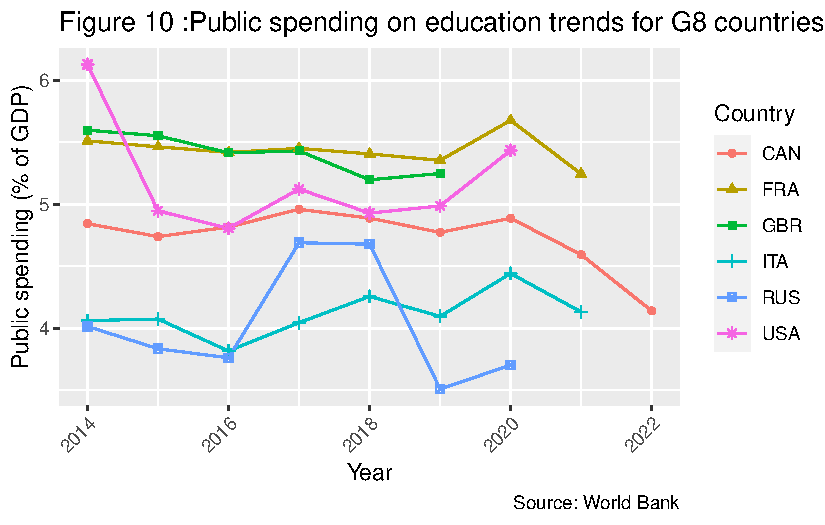
\includegraphics{Projet-BM_files/figure-pdf/unnamed-chunk-21-1.pdf}

Focusing solely on the G8 countries, we have assigned a color to each
country, showing that the United States (pink), France (yellow) and
Great Britain (green) are the countries that spend the most on
education. We can see that USA's public spending remains around 5,5\% of
the GDP compared to Italy with 4,1 of GDP. So, if we take the general
trend into account, we can see that for the selected countries we have a
drop in public spending on education. Moreover, we don't have any
information about public spending on education in Russia for 2021 and
2022.

\hypertarget{unemployement-rate-in-the-developped-countries-g8-countries}{%
\subsubsection{2) Unemployement rate in the developped countries : G8
countries}\label{unemployement-rate-in-the-developped-countries-g8-countries}}

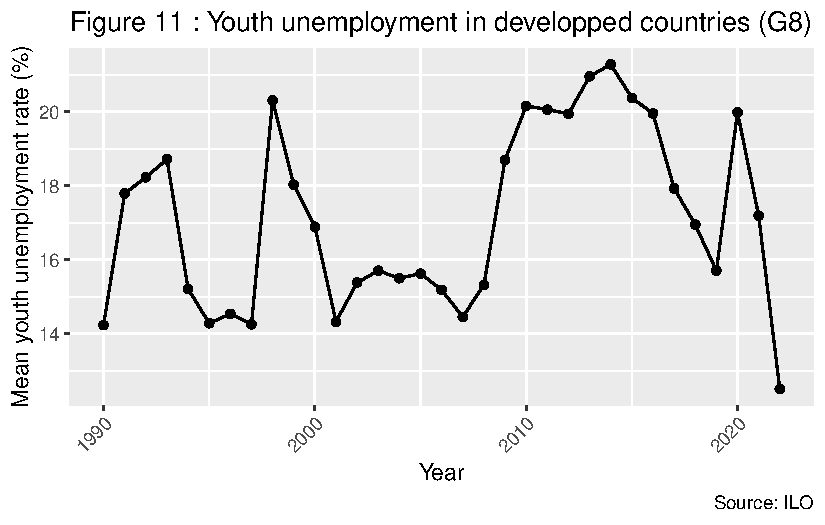
\includegraphics{Projet-BM_files/figure-pdf/unnamed-chunk-22-1.pdf}

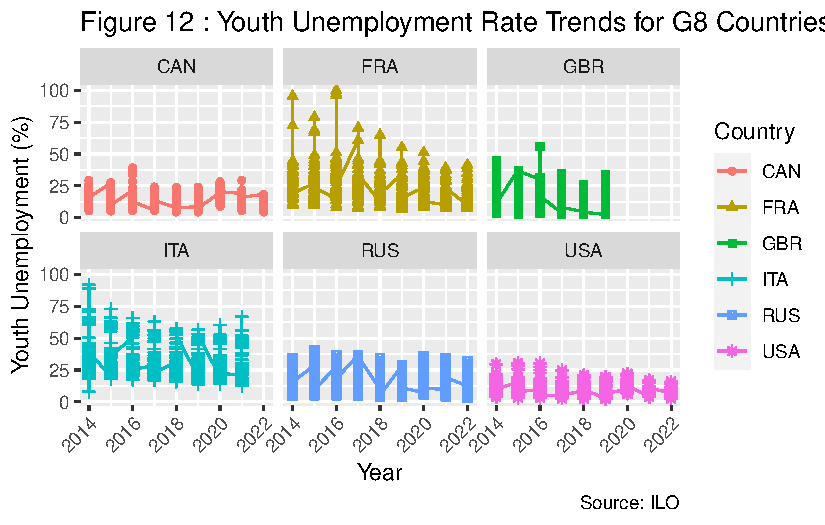
\includegraphics{Projet-BM_files/figure-pdf/unnamed-chunk-23-1.pdf}

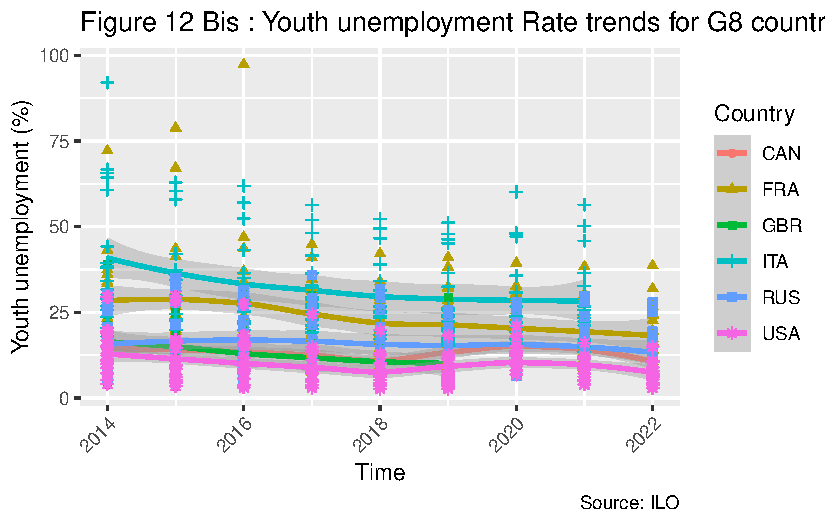
\includegraphics{Projet-BM_files/figure-pdf/unnamed-chunk-24-1.pdf}

This pair of graphs allows us to compare the trends in youth
unemployment rates among G8 countries. The United States has the lowest
youth unemployment rate.

\hypertarget{youth-unemployment-according-to-public-spending-for-g8-countries}{%
\subsubsection{3) Youth unemployment according to Public spending for G8
countries}\label{youth-unemployment-according-to-public-spending-for-g8-countries}}

\hypertarget{a-general-observations-according-to-education-level-and-sex}{%
\paragraph{a) general observations according to education level and
sex}\label{a-general-observations-according-to-education-level-and-sex}}

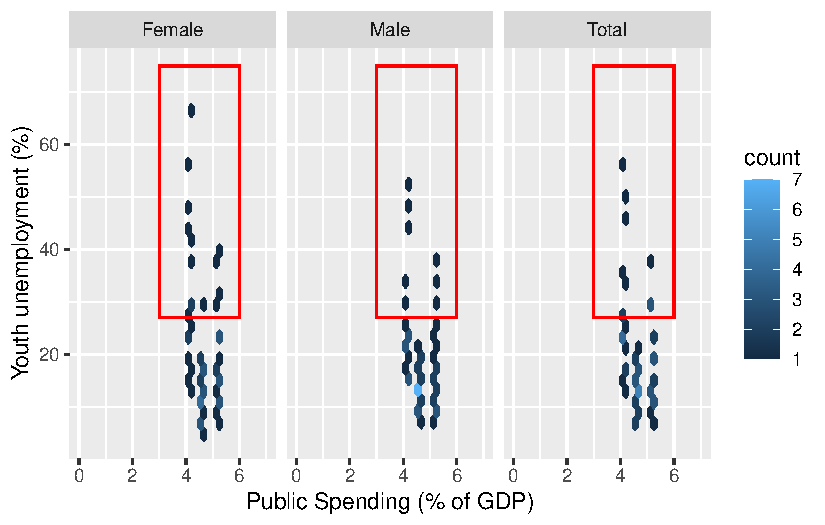
\includegraphics{Projet-BM_files/figure-pdf/unnamed-chunk-25-1.pdf}

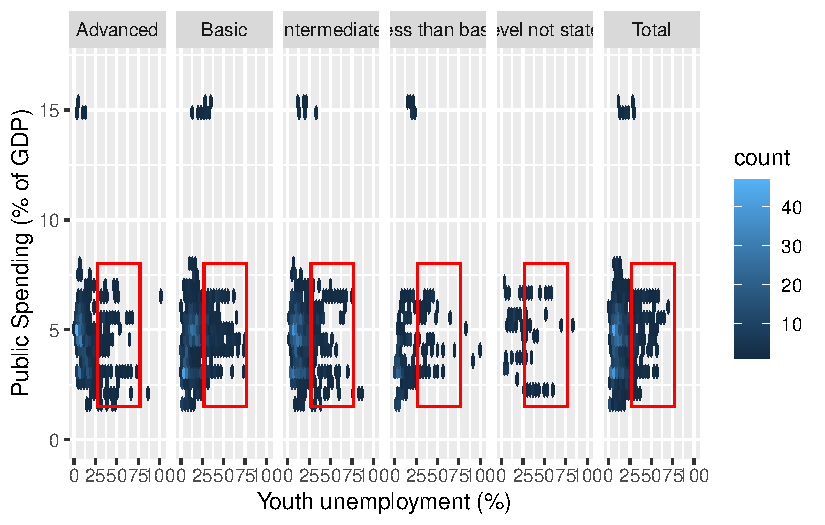
\includegraphics{Projet-BM_files/figure-pdf/unnamed-chunk-25-2.pdf}

When we examine public spending and the youth unemployment rate by
gender for G8 countries, we can observe that, for the G8 countries, any
increase in public spending results in a reduction in the unemployment
rate, although this result is less evident for women.

\hypertarget{b-according-to-education-and-age-range}{%
\paragraph{b) according to education and age
range}\label{b-according-to-education-and-age-range}}

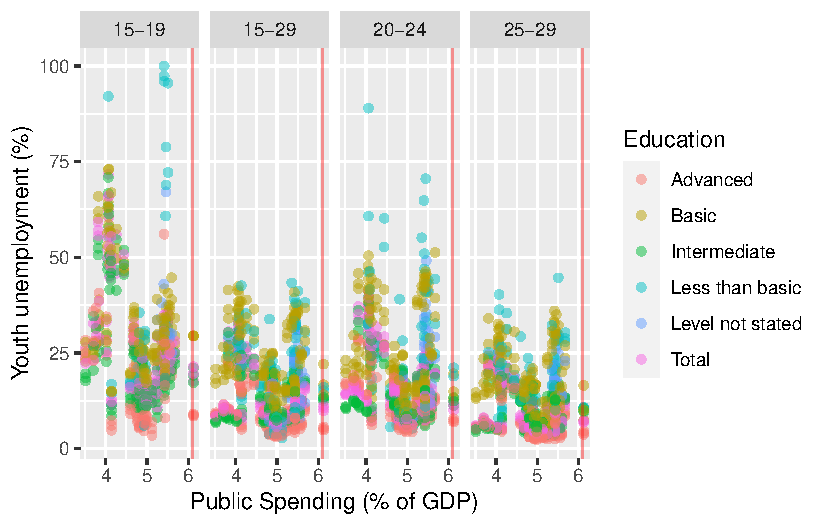
\includegraphics{Projet-BM_files/figure-pdf/unnamed-chunk-26-1.pdf}

For the 15-19 age group, we can see that the increase in public spending
allocated to education has a more significant effect for a higher level
of education.

\hypertarget{iii---public-spending-in-developping-countries---on-the-african-continent}{%
\subsubsection{III - Public spending in developping countries - on the
African
continent}\label{iii---public-spending-in-developping-countries---on-the-african-continent}}

We have previously observed how African countries have the highest youth
unemployment ratios whilst not having the lowest public spending in
education. It is therefore necessary to have a look at trends and
causality between public expenditure and unemployment in the region.

We'll be looking at public spending trends in Africa such as : Africa
Eastern and Southern (AFE), Burundi (BDI), Burkina Faso (BFA), Belize
(BLZ), Central African Republic (CAF), Congo - Democratic Republic of
Congo (COD), etc..

\hypertarget{a-general-trends-in-public-spending-on-education-of-gdp}{%
\paragraph{a) General trends in public spending on education (\% of
GDP)}\label{a-general-trends-in-public-spending-on-education-of-gdp}}

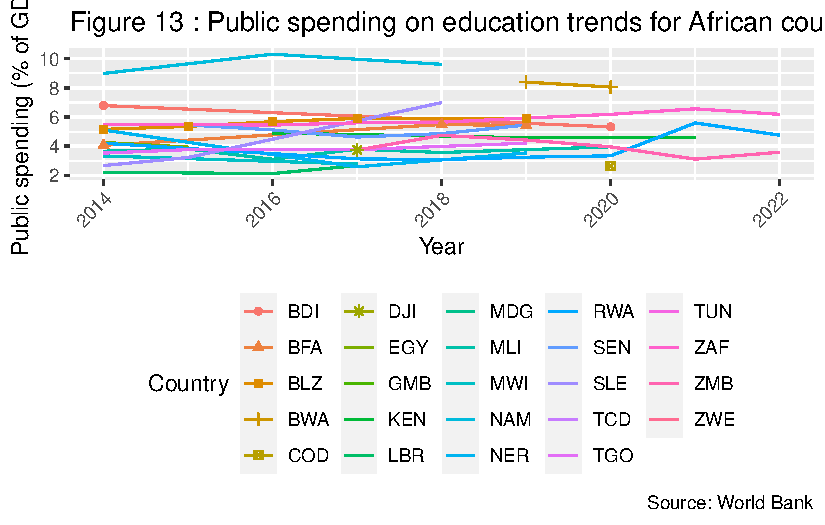
\includegraphics{Projet-BM_files/figure-pdf/unnamed-chunk-27-1.pdf}

In comparison with the graph showing the evolution of the share of
public expenditure in GDP for the G8 countries (Figure 10), we still
observe disparities between countries, that are even more pronounced for
African countries going up to nearly 8 percentage points difference
(Namibia vs Madagascar). The disparity is even more pronounced with
Namibia's higher than 8\% of GDP public spending in education.

\hypertarget{general-trends-in-unemployement-rate}{%
\subsubsection{2) General trends in unemployement
rate}\label{general-trends-in-unemployement-rate}}

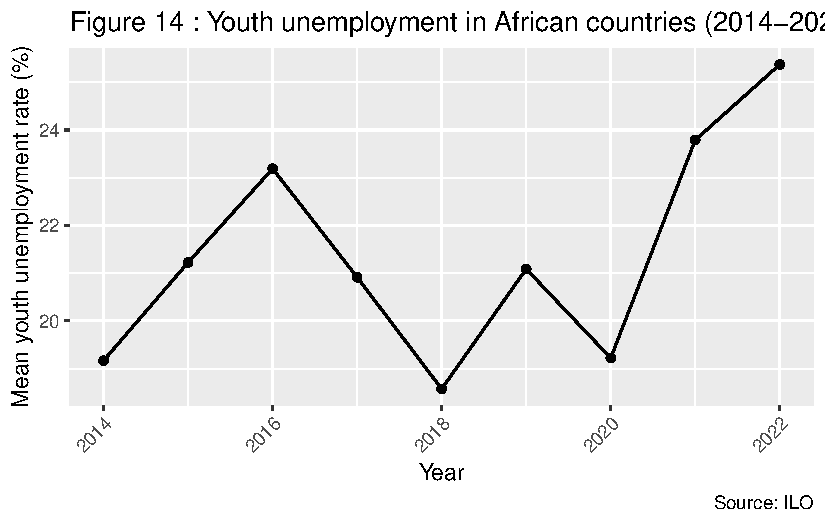
\includegraphics{Projet-BM_files/figure-pdf/unnamed-chunk-28-1.pdf}

Youth unemployment in Africa is higher than in the rest of the world,
with a notable resurge since 2020. That may be caused by the current
dept problems African countries have faced that have only worsened with
the COVID-19 crisis. Dept problems allow for budget constraints as the
government is focused on reducing their dept. This may lead to a
reduction of public spending in education (not very observable in the
previous graph because of missing values) and lead to higher
unemployment. This will be latered studied though regression tests.

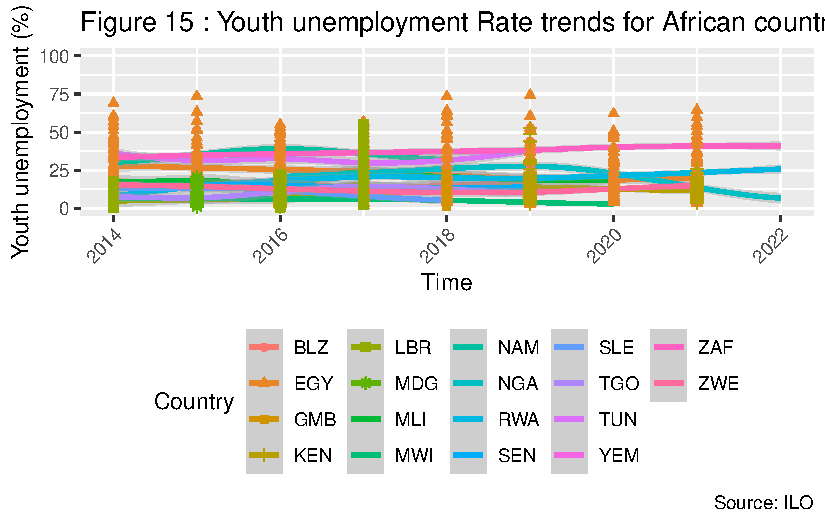
\includegraphics{Projet-BM_files/figure-pdf/unnamed-chunk-29-1.pdf}

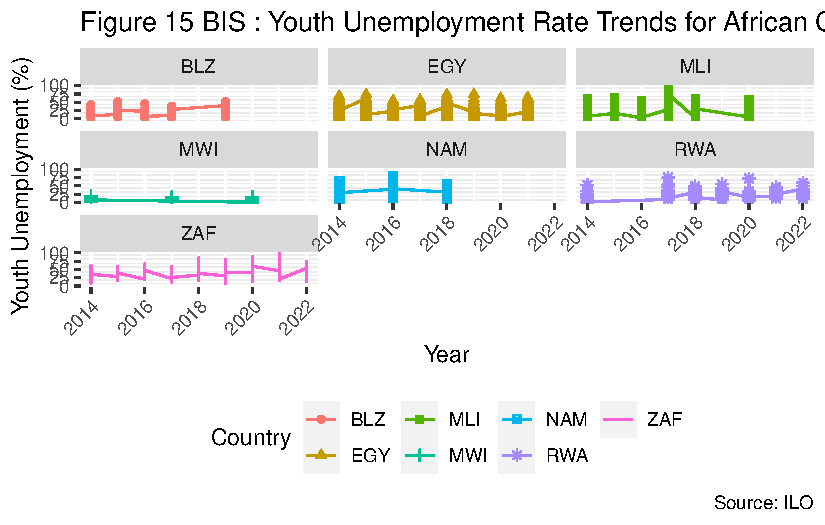
\includegraphics{Projet-BM_files/figure-pdf/unnamed-chunk-30-1.pdf}

Once again, we observe a great disparity in youth unemployment between
the countries we have observed. We can see that Malawi has a very low
unemployment rates, without having a particularly high public
expenditure (cf.~figure 13). Public spending therefore impacts these
countries very differently depending on the institutions and policies
established.

\hypertarget{impact-of-public-spending-on-education-level-on-african-countries}{%
\subsubsection{3) Impact of public spending on education level on
African
countries}\label{impact-of-public-spending-on-education-level-on-african-countries}}

\hypertarget{a-general-observations-1}{%
\paragraph{a) general observations}\label{a-general-observations-1}}

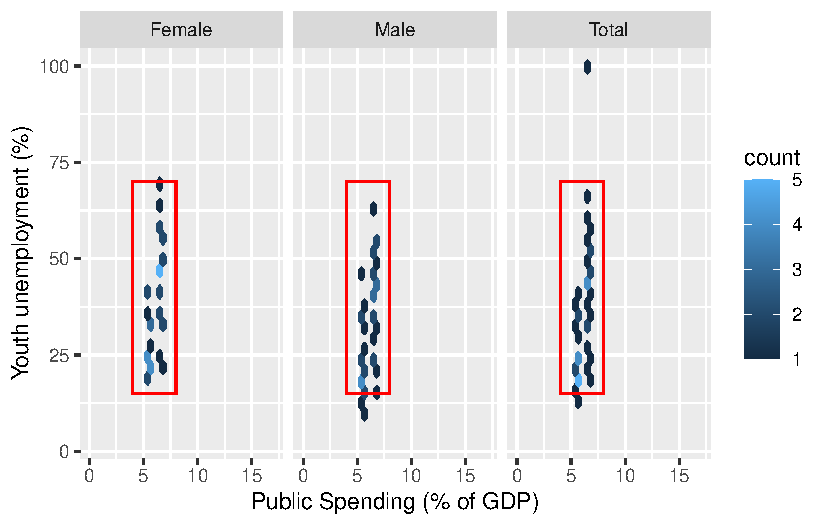
\includegraphics{Projet-BM_files/figure-pdf/unnamed-chunk-31-1.pdf}

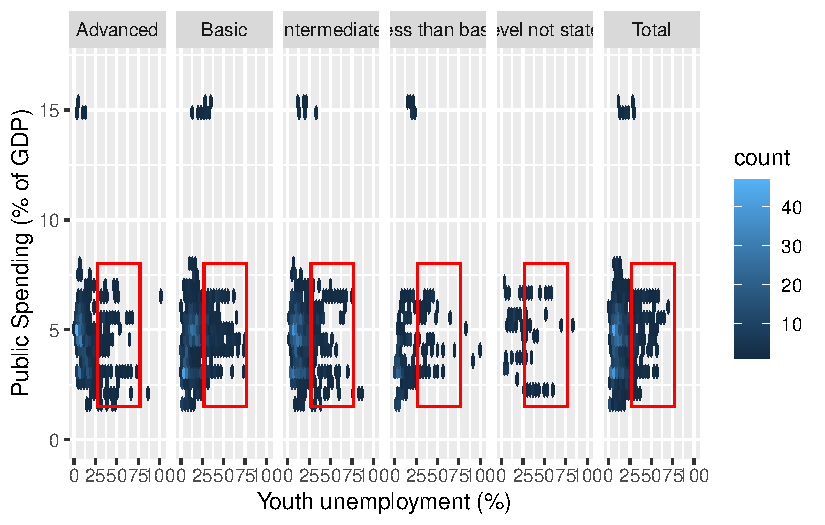
\includegraphics{Projet-BM_files/figure-pdf/unnamed-chunk-31-2.pdf}

Once again, women tend to have higher unemployment rates, the disparity
is however lower than the g8 countries. But the g8 countries still have
lower youth unemployment rates than the African countries for both
sexes.

\hypertarget{b-according-to-education}{%
\paragraph{b) according to education}\label{b-according-to-education}}

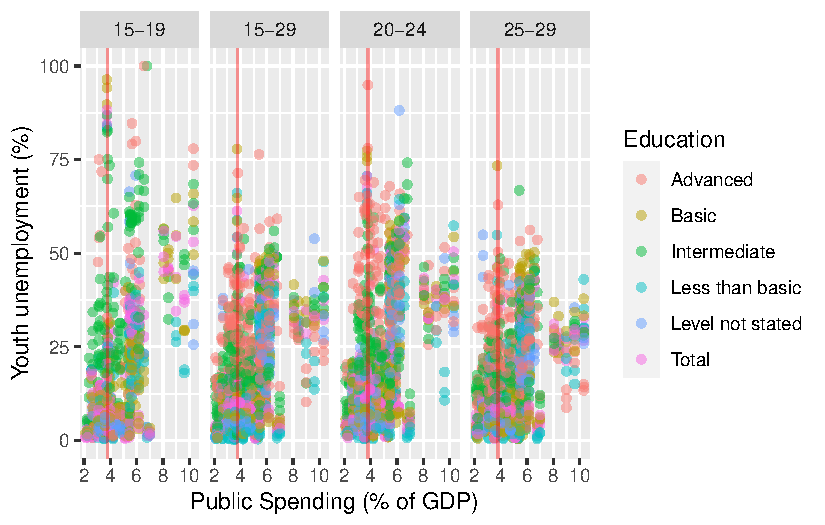
\includegraphics{Projet-BM_files/figure-pdf/unnamed-chunk-32-1.pdf}

In this graph we can see that, in the case of African countries,
advanced level of education still lead to high unemployment rate even
when public spending in education hovers around 6-7\% of GDP. This is
still true for higher age ranges such as 25-29. This matter worsens in
the case of low public expenditure. We have taken for example a public
spendinf og 7.8\% of GDP (red vertical line) where we can observe high
unemployment rates for teh 20-24 and 24-29 age ranges. This might be
understood by an inefficiency of public spending that we will test with
a linear regression.

\hypertarget{statistical-test-linear-regression-instrumental-variables}{%
\section{Statistical test, linear regression, instrumental
variables}\label{statistical-test-linear-regression-instrumental-variables}}

The second part being a more descriptive part highlighting the major
trends in the world and in specific geographical areas, such as Africa
in our case. In this last part of our project we will look carefully at
the different links that education spending and the youth unemployment
rate have between them. For this we will carry out statistical tests
such as the chi-square law, linear regressions.

Instrumental variables are used to solve the endogeneity problem in
econometric models. We want to run a linear regression looking at the
impact of education spending on the youth unemployment rate. In our
project, we will use education expenditure as the explanatory variable
and the youth unemployment rate as the explained variable.

To deepen our analysis, we will use instrumental variables, which are
variables used to solve the endogeneity problem in econometric models.
Endogeneity can arise when the explanatory variable is correlated with
model errors, which can bias estimation results. Instrumental variables
are therefore used to isolate the uncorrelated variation of the
explanatory variable and use it as a proxy for that variable.

For the purposes of this project, we can therefore use the following
instrumental variables: total government expenditure, number of schools
per capita and population growth rate. This allows us to see whether
these variables are not correlated directly with the youth unemployment
rate, but are correlated directly with education spending.

\hypertarget{i-correlation-test-for-the-world}{%
\subsection{I) Correlation test for the
world}\label{i-correlation-test-for-the-world}}

To understand the relationship between public spending on education and
the youth unemployment rate, we will perform a correlation analysis.

\hypertarget{correlation}{%
\subsubsection{1) Correlation}\label{correlation}}

\begin{verbatim}

    Pearson's product-moment correlation

data:  dep_chomage$`Public Spending (% of GDP)` and dep_chomage$`Youth unemployment (%)`
t = 1.3988, df = 79771, p-value = 0.1619
alternative hypothesis: true correlation is not equal to 0
95 percent confidence interval:
 -0.001987041  0.011891399
sample estimates:
        cor 
0.004952417 
\end{verbatim}

\hypertarget{linear-regression}{%
\subsubsection{2) Linear Regression}\label{linear-regression}}

\begin{verbatim}

Call:
lm(formula = `Youth unemployment (%)` ~ `Public Spending (% of GDP)`, 
    data = dep_chomage)

Residuals:
    Min      1Q  Median      3Q     Max 
-17.170 -10.051  -4.024   6.236  82.709 

Coefficients:
                             Estimate Std. Error t value Pr(>|t|)    
(Intercept)                  17.13004    0.16160 106.000   <2e-16 ***
`Public Spending (% of GDP)`  0.04616    0.03300   1.399    0.162    
---
Signif. codes:  0 '***' 0.001 '**' 0.01 '*' 0.05 '.' 0.1 ' ' 1

Residual standard error: 13.91 on 79771 degrees of freedom
  (29215 observations deleted due to missingness)
Multiple R-squared:  2.453e-05, Adjusted R-squared:  1.199e-05 
F-statistic: 1.957 on 1 and 79771 DF,  p-value: 0.1619
\end{verbatim}

\hypertarget{regression-model}{%
\paragraph{Regression Model}\label{regression-model}}

The simple linear regression model can be represented as:

{[} ~Y\_\{t\} = ß\_\{0\} + ß\_\{1\}X\_\{t\} + \varepsilon\_\{t\} {]}

where: - (Y\_\{t\}): Youth unemployment rate at time (t). -
(\beta\emph{\{0\}): Intercept term. - (\beta}\{1\}): Coefficient for the
variable (X\_\{t\}). - (X\_\{t\}): Public spending variable at time (t).
- (\epsilon\_\{t\}): Error term.

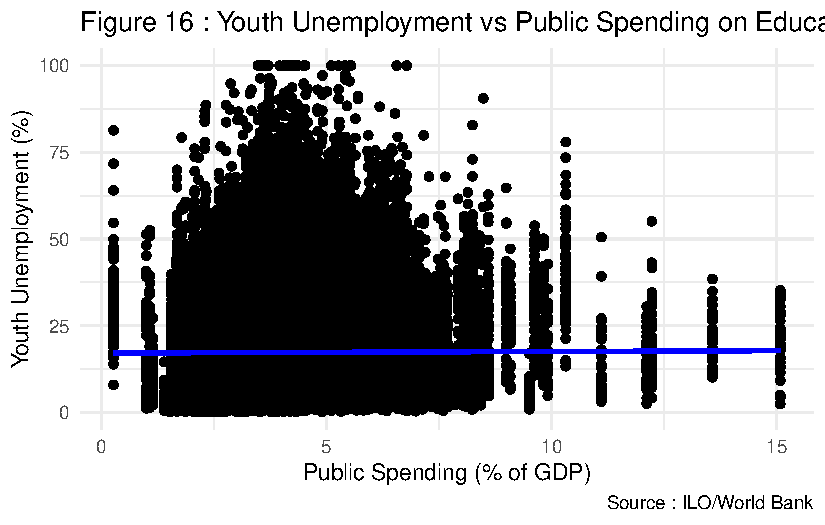
\includegraphics{Projet-BM_files/figure-pdf/unnamed-chunk-35-1.pdf}

When we take the global data, the regression line is almost straight, or
slightly decreasing, this may suggest that for every increase (decrease)
in education spending, the youth unemployment rate decreases (or
increases) by constant manner. Furthermore, this may also suggest an
absence of causal link between the two variables.

\hypertarget{chi-deux-test}{%
\subsubsection{3) Chi deux test}\label{chi-deux-test}}

\begin{verbatim}

    Pearson's Chi-squared test

data:  table(dep_chomage$`Youth unemployment (%)`, dep_chomage$sex)
X-squared = 78883, df = 78334, p-value = 0.08284
\end{verbatim}

The p-value of 0.03145 is less than the common significance level of
0.05. With a p-value below 0.05, we must reject the null hypothesis. In
the context of a chi-square test for independence, this result suggests
that there is evidence of an association between the variables Youth
unemployment (\%) and gender. The association is considered
statistically significant.

\hypertarget{ii-statistical-test---g8-countries}{%
\subsection{II) Statistical test - G8
countries}\label{ii-statistical-test---g8-countries}}

\hypertarget{correlation-test}{%
\subsubsection{1) Correlation test}\label{correlation-test}}

\begin{verbatim}

    Pearson's product-moment correlation

data:  dep_chomage_g8_filtered$`Public Spending (% of GDP)` and dep_chomage_g8_filtered$`Youth unemployment (%)`
t = -7.988, df = 2470, p-value = 2.083e-15
alternative hypothesis: true correlation is not equal to 0
95 percent confidence interval:
 -0.1968824 -0.1200167
sample estimates:
     cor 
-0.15869 
\end{verbatim}

\hypertarget{linear-regression---g8-countries}{%
\subsubsection{2) Linear regression - G8
countries}\label{linear-regression---g8-countries}}

\begin{verbatim}

Call:
lm(formula = `Youth unemployment (%)` ~ `Public Spending (% of GDP)`, 
    data = dep_chomage_g8)

Residuals:
    Min      1Q  Median      3Q     Max 
-18.601  -8.162  -2.103   5.608  82.604 

Coefficients:
                             Estimate Std. Error t value Pr(>|t|)    
(Intercept)                   29.8130     0.8409   35.45   <2e-16 ***
`Public Spending (% of GDP)`  -2.2914     0.1630  -14.06   <2e-16 ***
---
Signif. codes:  0 '***' 0.001 '**' 0.01 '*' 0.05 '.' 0.1 ' ' 1

Residual standard error: 11.18 on 6821 degrees of freedom
  (876 observations deleted due to missingness)
Multiple R-squared:  0.02816,   Adjusted R-squared:  0.02802 
F-statistic: 197.7 on 1 and 6821 DF,  p-value: < 2.2e-16
\end{verbatim}

\begin{verbatim}
     Correlation Coefficient      P-Value
[1,]                -0.15869 2.083238e-15
\end{verbatim}

The correlation test provides valuable insights into the strength and
direction of the linear relationship between public spending on
education and the youth unemployment rate. The correlation coefficient
and p-value help us assess the statistical significance of the observed
correlation. In this case, with a negative correlation coefficient
between public spending (\% of GDP) and youth unemployment (\%), this
suggests that there could be a trend where higher levels of public
spending are associated with lower rates of youth unemployment, and vice
versa.

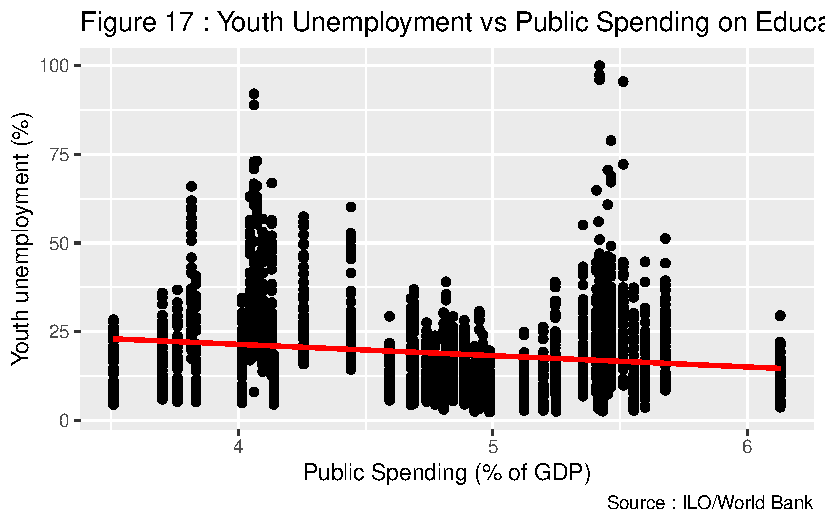
\includegraphics{Projet-BM_files/figure-pdf/unnamed-chunk-40-1.pdf}

The scatter plot with a fitted line visually represents the correlation
between public spending and the youth unemployment rate. The blue line
indicates the linear regression fit.

The correlation test and visualization help us understand if there is a
significant correlation between public spending on education and the
youth unemployment rate. The correlation coefficient close to 1 or -1
indicates a strong relationship, while a p-value less than 0.05 suggests
statistical significance.

\hypertarget{iii-statistical-test---african-countries}{%
\subsection{III) Statistical test - African
countries}\label{iii-statistical-test---african-countries}}

\hypertarget{correlation-test-1}{%
\subsubsection{1) Correlation test}\label{correlation-test-1}}

\begin{verbatim}

    Pearson's product-moment correlation

data:  dep_chomage_g8_filtered$`Public Spending (% of GDP)` and dep_chomage_g8_filtered$`Youth unemployment (%)`
t = -7.988, df = 2470, p-value = 2.083e-15
alternative hypothesis: true correlation is not equal to 0
95 percent confidence interval:
 -0.1968824 -0.1200167
sample estimates:
     cor 
-0.15869 
\end{verbatim}

\hypertarget{linear-regression---african-countries}{%
\subsubsection{2) Linear regression - African
countries}\label{linear-regression---african-countries}}

\begin{verbatim}

Call:
lm(formula = `Youth unemployment (%)` ~ `Public Spending (% of GDP)`, 
    data = dep_chomage_afr_unemployment)

Residuals:
    Min      1Q  Median      3Q     Max 
-27.387 -10.413  -2.987   8.085  78.895 

Coefficients:
                             Estimate Std. Error t value Pr(>|t|)    
(Intercept)                    1.6709     0.7125   2.345   0.0191 *  
`Public Spending (% of GDP)`   3.7838     0.1388  27.268   <2e-16 ***
---
Signif. codes:  0 '***' 0.001 '**' 0.01 '*' 0.05 '.' 0.1 ' ' 1

Residual standard error: 14.61 on 3793 degrees of freedom
  (1121 observations deleted due to missingness)
Multiple R-squared:  0.1639,    Adjusted R-squared:  0.1637 
F-statistic: 743.6 on 1 and 3793 DF,  p-value: < 2.2e-16
\end{verbatim}

\begin{verbatim}
     Correlation Coefficient      P-Value
[1,]                -0.15869 2.083238e-15
\end{verbatim}

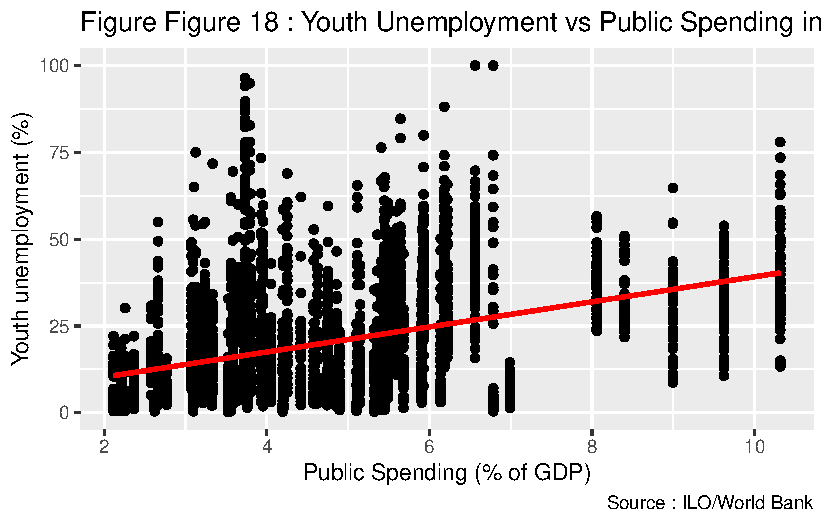
\includegraphics{Projet-BM_files/figure-pdf/unnamed-chunk-44-1.pdf}

When we take all African countries together, we can see a different
correlation to the one previously calculated. In fact, it's positive,
suggesting that the higher the public spending, the higher the youth
unemployment rate.

This clearly validates our previous observation concerning African
countries, and might be due to corruption or inefficient policies
(typically dealing with lack of efficiency as a demand problem instead
of a supply/quality problem).

\hypertarget{iv-add-instrumentales-variables-stability-of-countries-for-example}{%
\subsection{IV) Add instrumentales variables : stability of countries
for
example}\label{iv-add-instrumentales-variables-stability-of-countries-for-example}}

To further enhance the analysis, we can add additional explanatory
variables such as gender and education level to our regression models.
We will only do this for the G8 countries.

\hypertarget{linear-regression-with-education-and-sex-for-g8-countries}{%
\subsubsection{1) Linear regression with education and sex for G8
countries}\label{linear-regression-with-education-and-sex-for-g8-countries}}

\hypertarget{a-education}{%
\paragraph{a) Education}\label{a-education}}

\begin{verbatim}

Call:
lm(formula = `Youth unemployment (%)` ~ `Public Spending (% of GDP)` + 
    Education, data = dep_chomage_g8_filtered)

Residuals:
    Min      1Q  Median      3Q     Max 
-21.206  -7.498  -2.107   5.238  77.201 

Coefficients:
                             Estimate Std. Error t value Pr(>|t|)    
(Intercept)                   29.4414     1.8383  16.015  < 2e-16 ***
`Public Spending (% of GDP)`  -3.7286     0.3684 -10.120  < 2e-16 ***
EducationBasic                13.9602     0.7023  19.878  < 2e-16 ***
EducationIntermediate          4.8812     0.7023   6.950 4.65e-12 ***
EducationLess than basic      13.5629     0.8485  15.984  < 2e-16 ***
EducationLevel not stated     13.2016     1.2762  10.345  < 2e-16 ***
EducationTotal                 5.4999     0.7023   7.831 7.12e-15 ***
---
Signif. codes:  0 '***' 0.001 '**' 0.01 '*' 0.05 '.' 0.1 ' ' 1

Residual standard error: 11.21 on 2465 degrees of freedom
  (260 observations deleted due to missingness)
Multiple R-squared:  0.2014,    Adjusted R-squared:  0.1995 
F-statistic: 103.6 on 6 and 2465 DF,  p-value: < 2.2e-16
\end{verbatim}

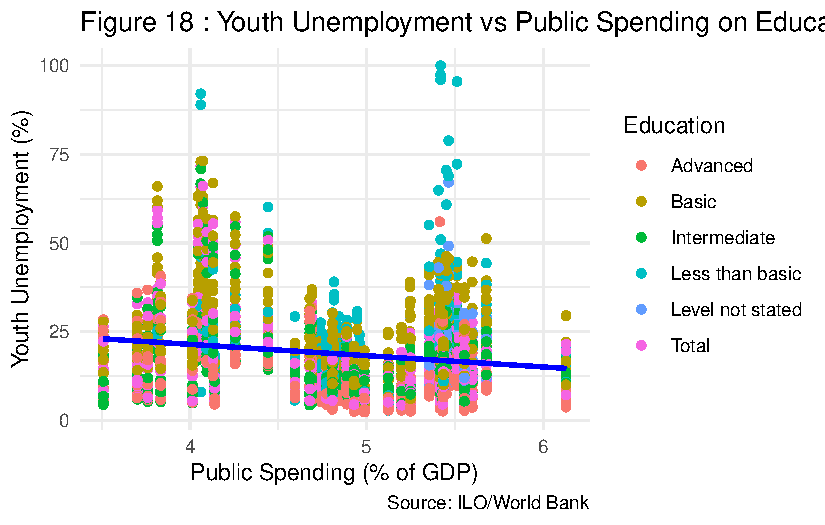
\includegraphics{Projet-BM_files/figure-pdf/unnamed-chunk-45-1.pdf}

\hypertarget{b-by-sex}{%
\paragraph{b) By sex}\label{b-by-sex}}

\begin{verbatim}

Call:
lm(formula = `Youth unemployment (%)` ~ `Public Spending (% of GDP)` + 
    sex, data = dep_chomage_g8_filtered)

Residuals:
    Min      1Q  Median      3Q     Max 
-18.010  -8.986  -2.503   5.852  82.475 

Coefficients:
                             Estimate Std. Error t value Pr(>|t|)    
(Intercept)                   34.7515     1.9714  17.628  < 2e-16 ***
`Public Spending (% of GDP)`  -3.1789     0.3980  -7.987  2.1e-15 ***
sexMale                       -1.1625     0.6126  -1.898   0.0579 .  
sexTotal                      -0.7227     0.6096  -1.185   0.2359    
---
Signif. codes:  0 '***' 0.001 '**' 0.01 '*' 0.05 '.' 0.1 ' ' 1

Residual standard error: 12.37 on 2468 degrees of freedom
  (260 observations deleted due to missingness)
Multiple R-squared:  0.02663,   Adjusted R-squared:  0.02545 
F-statistic: 22.51 on 3 and 2468 DF,  p-value: 2.255e-14
\end{verbatim}

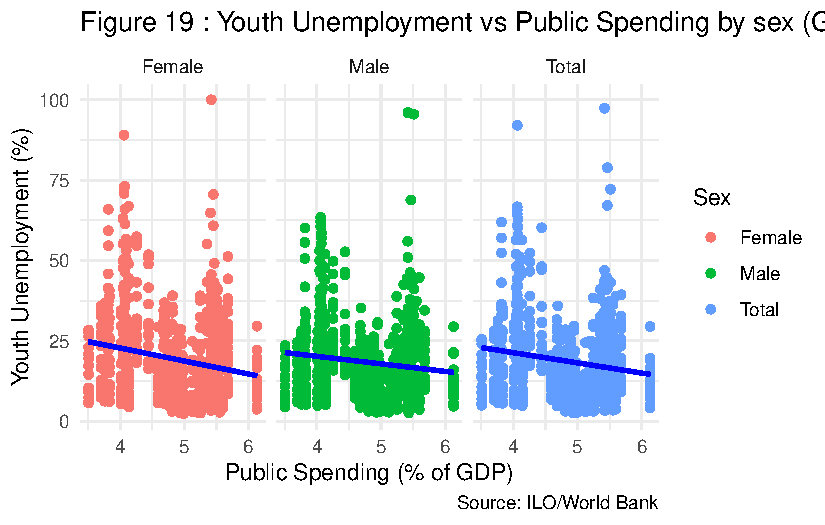
\includegraphics{Projet-BM_files/figure-pdf/unnamed-chunk-46-1.pdf}

\hypertarget{c-education-and-sex}{%
\paragraph{c) Education and sex}\label{c-education-and-sex}}

\hypertarget{regression-model-for-g8-countries}{%
\paragraph{Regression Model for G8
countries}\label{regression-model-for-g8-countries}}

The simple linear regression model can be represented as:

{[} ~Y\_\{t\} = ß\_\{0\} + ß\_\{1\}X\_\{t\} + ß\{2\}\emph{Education +
ß\{3\}}sex \varepsilon\emph{\{t\} \varepsilon}\{t\} {]}

where: - (Y\_\{t\}): Youth unemployment rate at time (t). -
(\beta\emph{\{0\}): Intercept term. - (\beta}\{1\}): Coefficient for the
variable (X\_\{t\}). - (X\_\{t\}): Public spending variable at time (t).
- (\epsilon\_\{t\}): Error term.

\begin{verbatim}

Call:
lm(formula = `Youth unemployment (%)` ~ `Public Spending (% of GDP)` + 
    sex, data = dep_chomage_g8_filtered)

Residuals:
    Min      1Q  Median      3Q     Max 
-18.010  -8.986  -2.503   5.852  82.475 

Coefficients:
                             Estimate Std. Error t value Pr(>|t|)    
(Intercept)                   34.7515     1.9714  17.628  < 2e-16 ***
`Public Spending (% of GDP)`  -3.1789     0.3980  -7.987  2.1e-15 ***
sexMale                       -1.1625     0.6126  -1.898   0.0579 .  
sexTotal                      -0.7227     0.6096  -1.185   0.2359    
---
Signif. codes:  0 '***' 0.001 '**' 0.01 '*' 0.05 '.' 0.1 ' ' 1

Residual standard error: 12.37 on 2468 degrees of freedom
  (260 observations deleted due to missingness)
Multiple R-squared:  0.02663,   Adjusted R-squared:  0.02545 
F-statistic: 22.51 on 3 and 2468 DF,  p-value: 2.255e-14
\end{verbatim}

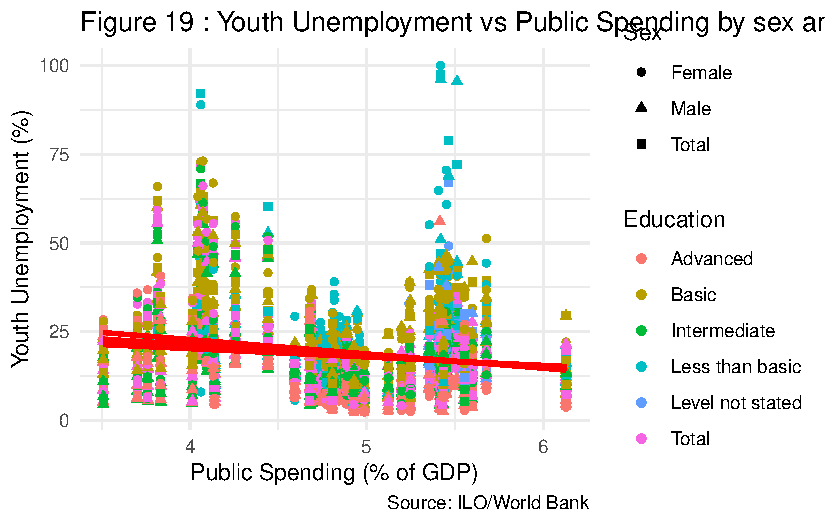
\includegraphics{Projet-BM_files/figure-pdf/unnamed-chunk-47-1.pdf}

After adding the Education and sex control variables we can see public
spending still has a negative impact on youth unemployment. Education is
therefore not the only factor of unemployment and public expenditure has
a direct impact on youth unemployment on the labor market.

\hypertarget{conclusion}{%
\section{Conclusion}\label{conclusion}}

Throughout our study we have observed general and more particular trends
in public spending in education and youth unemployment around the world.
By focusing on the G8 countries and African countries, and conduction
linear regressions and correlations trends we were able to understand
the various impacts of public spending on unemployment.

When it comes to the G8 countries, public spending has a negative impact
on youth unemployment highlighting the need to tackle issues on the
labor market through an educational approach. For the same amount of
public spending youth unemployment is higher for women. However the
difference between men and women decreases for higher public spending
making it a good approach to reducing inequalities on the labor market.
For different age groups and level of education, young people with low
education levels tend to have a high unemployment ratio as they may
still be in school. However, unemployment strongly decreases in higher
age ranges and for higher education levels. Public spending in education
can therefore tackle unemployment issues by allowing students to pursue
higher degrees allowing them to easily find jobs on the labor market.

When it comes to the African countries, public spending has a chocking
positive impact on youth unemployment highlighting. This perfectly
represents the lack of efficiency of public spending when it isn't
coupled with sufficient public policies and control. For the same amount
of public spending youth unemployment is higher for women.Contrary to G8
countries, this difference does not decrease with the increase of public
spending. There are still discrimination issues to be tackled on the
labor market through other policy tools. Unemployment is till quite high
even for advanced level of education and older age ranges, even for high
pubic spending, this only accentuates the inefficiency of public
spending when it is not well implemented.

In conclusion, our study underscores the strong disparities in the
impact of public spending in education on youth unemployment between G8
countries and African nations, emphasizing the critical need for
tailored policy interventions to address these global differences. Our
analysis therefore advocates for a nuanced understanding of the
relationship between public spending and youth unemployment, urging
policymakers to elaborate targeted approaches to optimize the impact of
public funds on labor market dynamics.

\hypertarget{annexe}{%
\section{Annexe}\label{annexe}}

\#\#Github repository The GitHub project can be found on:
\emph{https://github.com/GhinaMezher/project-BM}.git 2 collaborators can
be found on this public project.

\hypertarget{links-and-sources}{%
\subsection{Links and sources}\label{links-and-sources}}

We used the data base from the World Bank and International Labor
Organization that identifies the public spendings in education:
\emph{https://data.worldbank.org/indicator/SE.XPD.TOTL.GD.ZS?end=2022\&start=1970\&view=chart}
And for the data on youth unemployment rates depending on various
caracteristics we referred to the International Labor Organisation (ILO)
database: \emph{https://ilostat.ilo.org/fr/topics/youth/\#} \&
\emph{https://www.ilo.org/shinyapps/bulkexplorer27/?lang=fr\&id=POP\_3WAP\_SEX\_AGE\_EDU\_NB\_A}



\end{document}
